\documentclass[../relazione.tex]{subfiles}

\begin{document}
\section{Accessibilità}
	\begin{itemize}
		\item è stato scelto un font molto chiaro per permettere all'utente di leggere senza sforzi il contenuto
		\item si è cercato di mantenere la semplicità in ogni parte del sito, sia nel contenuto che nella presentazione
		\item inserire gli screenshot presenti nella cartella images/colorblindness
		\item malattie testate: deuteranopia, monochromacy, partialMonochromacy, protanopia, tritanopia
		\item indipendentemente dal tipo di malattia, il sito si presenta in maniera chiara e accessibile
		\item link: sono colorati di rosa salmone, però sono rafforzati dal grassetto proprio per renderli maggiormente distinguibili anche nel caso in cui l'utente non sia in grado di vedere il colore
		\item link: il caso più lampante per il nostro sito è la monochromacy: se non fossero in grassetto i link sarebbero difficilmente distinguibili dal resto del testo
		\item sono presenti molte paroli giapponesi all'interno del sito, per ovvii motivi: in ognuno di questi caso è stato definito l'attributo xml:lang="ja" tra gli attributi del tag all'interno il quale figuravano (ad es: strong) oppure tra gli attributi di uno span opportunamente piazzato -> per favorire la lettura del sito da parte dello screen reader
		\item presenti molte parole stranieri nel menù: giapponesi, francesi, tedesche, spagnole. Definito uno span opportuno per ognuna di queste occorrenze, con attributo xml:lang impostato sulla lingua richiesta -> per favorire la lettura del sito da parte dello screen reader
		\item title: definito dal particolare al generale
		\item javascript: nel caso in cui sia disattivato il sito degrada in maniera elegante
		\item javascript: se non è attivo, nella schermata del menu viene mostrata una lista di link per agevolare la navigazione all'interno della pagina stessa
		\item per quanto riguarda le form nella pagina private-menu.cgi ber bevande e cibi si è preferito semplificare la parte di presentazione pur di mantenere la validazione dell’XHTML e quindi mantenere un buon livello di accessibilità
		\item in tutte le form non è stata definita una legend perché ritenuta non necessaria
		\item segnalati in maniera elegante gli errori nelle form (aggiungere screenshot)
		\item Per essere accessibile un sito deve poter essere navigabile utilizzando solamente la tastiera. Ogni pagina è stata testata ed il risultato è che il sito è navigabile utilizzando \textit{Tab} ed \textit{Enter}, ad eccezione delle pagine menu.cgi e private-menu.cgi (parte pubblica e amministratore) con Javascript attivo. Infatti, nel caso in cui Javascript sia disattivato, il sito è navigabile totalmente da tastiera.
		\item Non sono stati utilizzati gli attributi \textit{tabindex} per i link in quanto il flusso logico del sito è semplice e lineare.
	\end{itemize}
	Immagini:
	\begin{figure}[H]
	\centering
		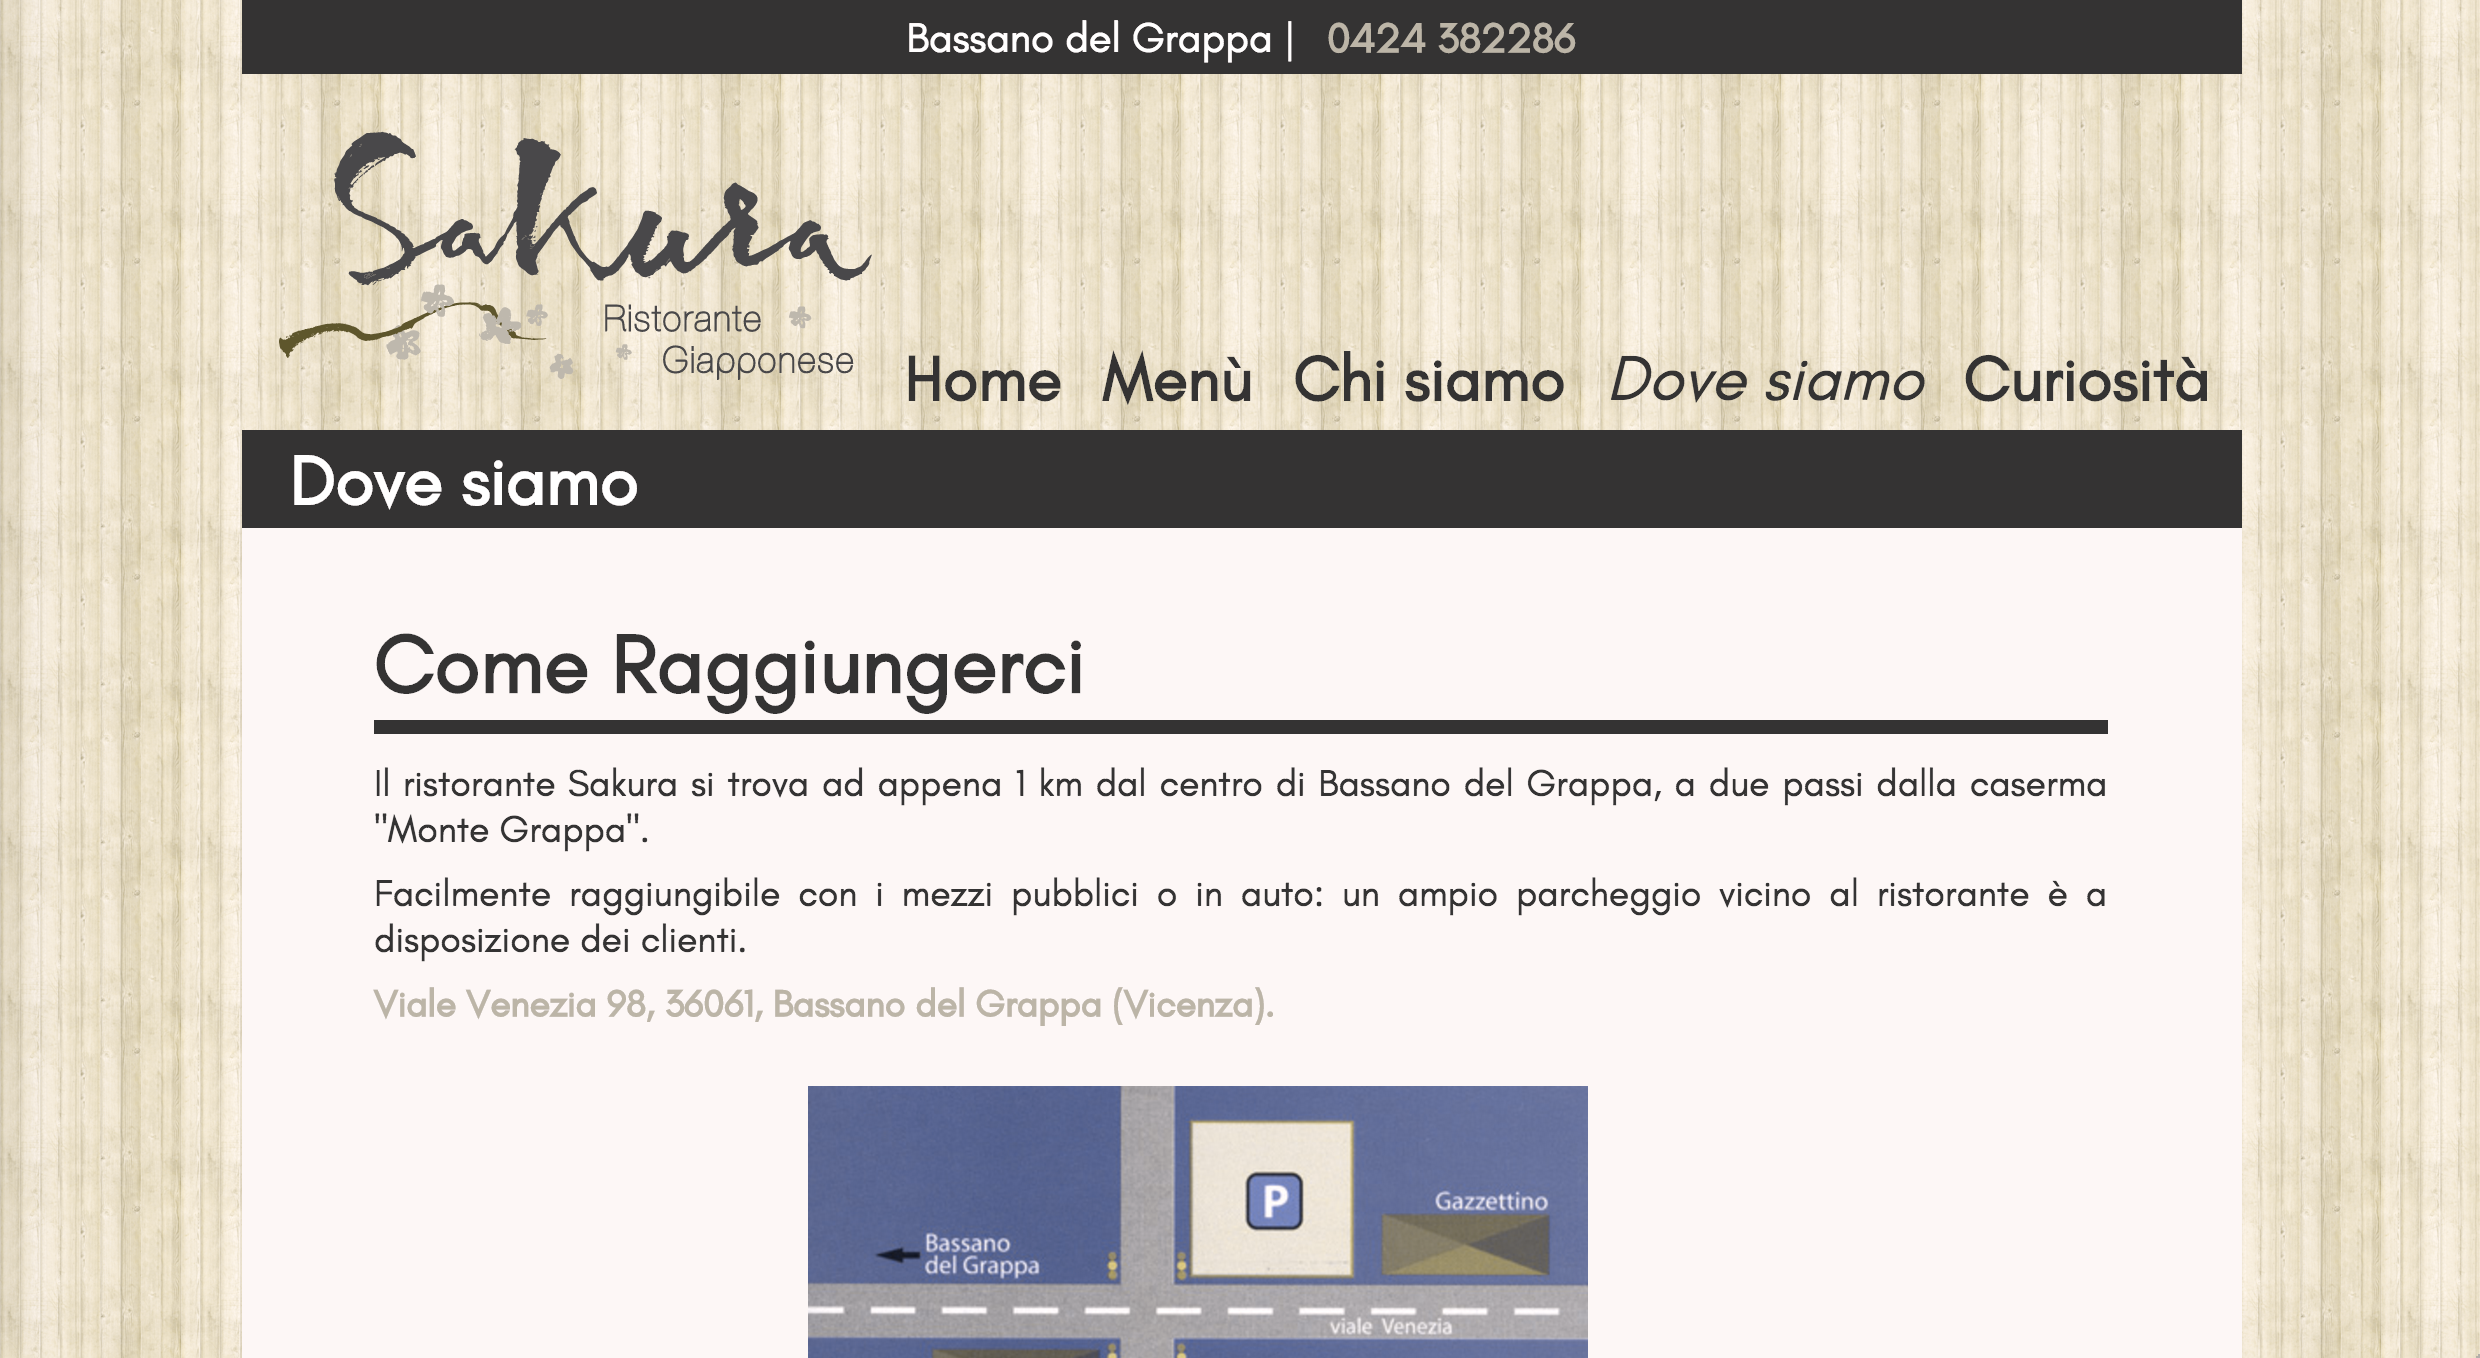
\includegraphics[width=\textwidth]{images/colorblindness/protanopia}
		\caption{Esempio di pagina vista da chi soffre di protanopia}
		\label{fig:Esempio di pagina vista da chi soffre di protanopia}
	\end{figure}
	\begin{figure}[H]
	\centering
		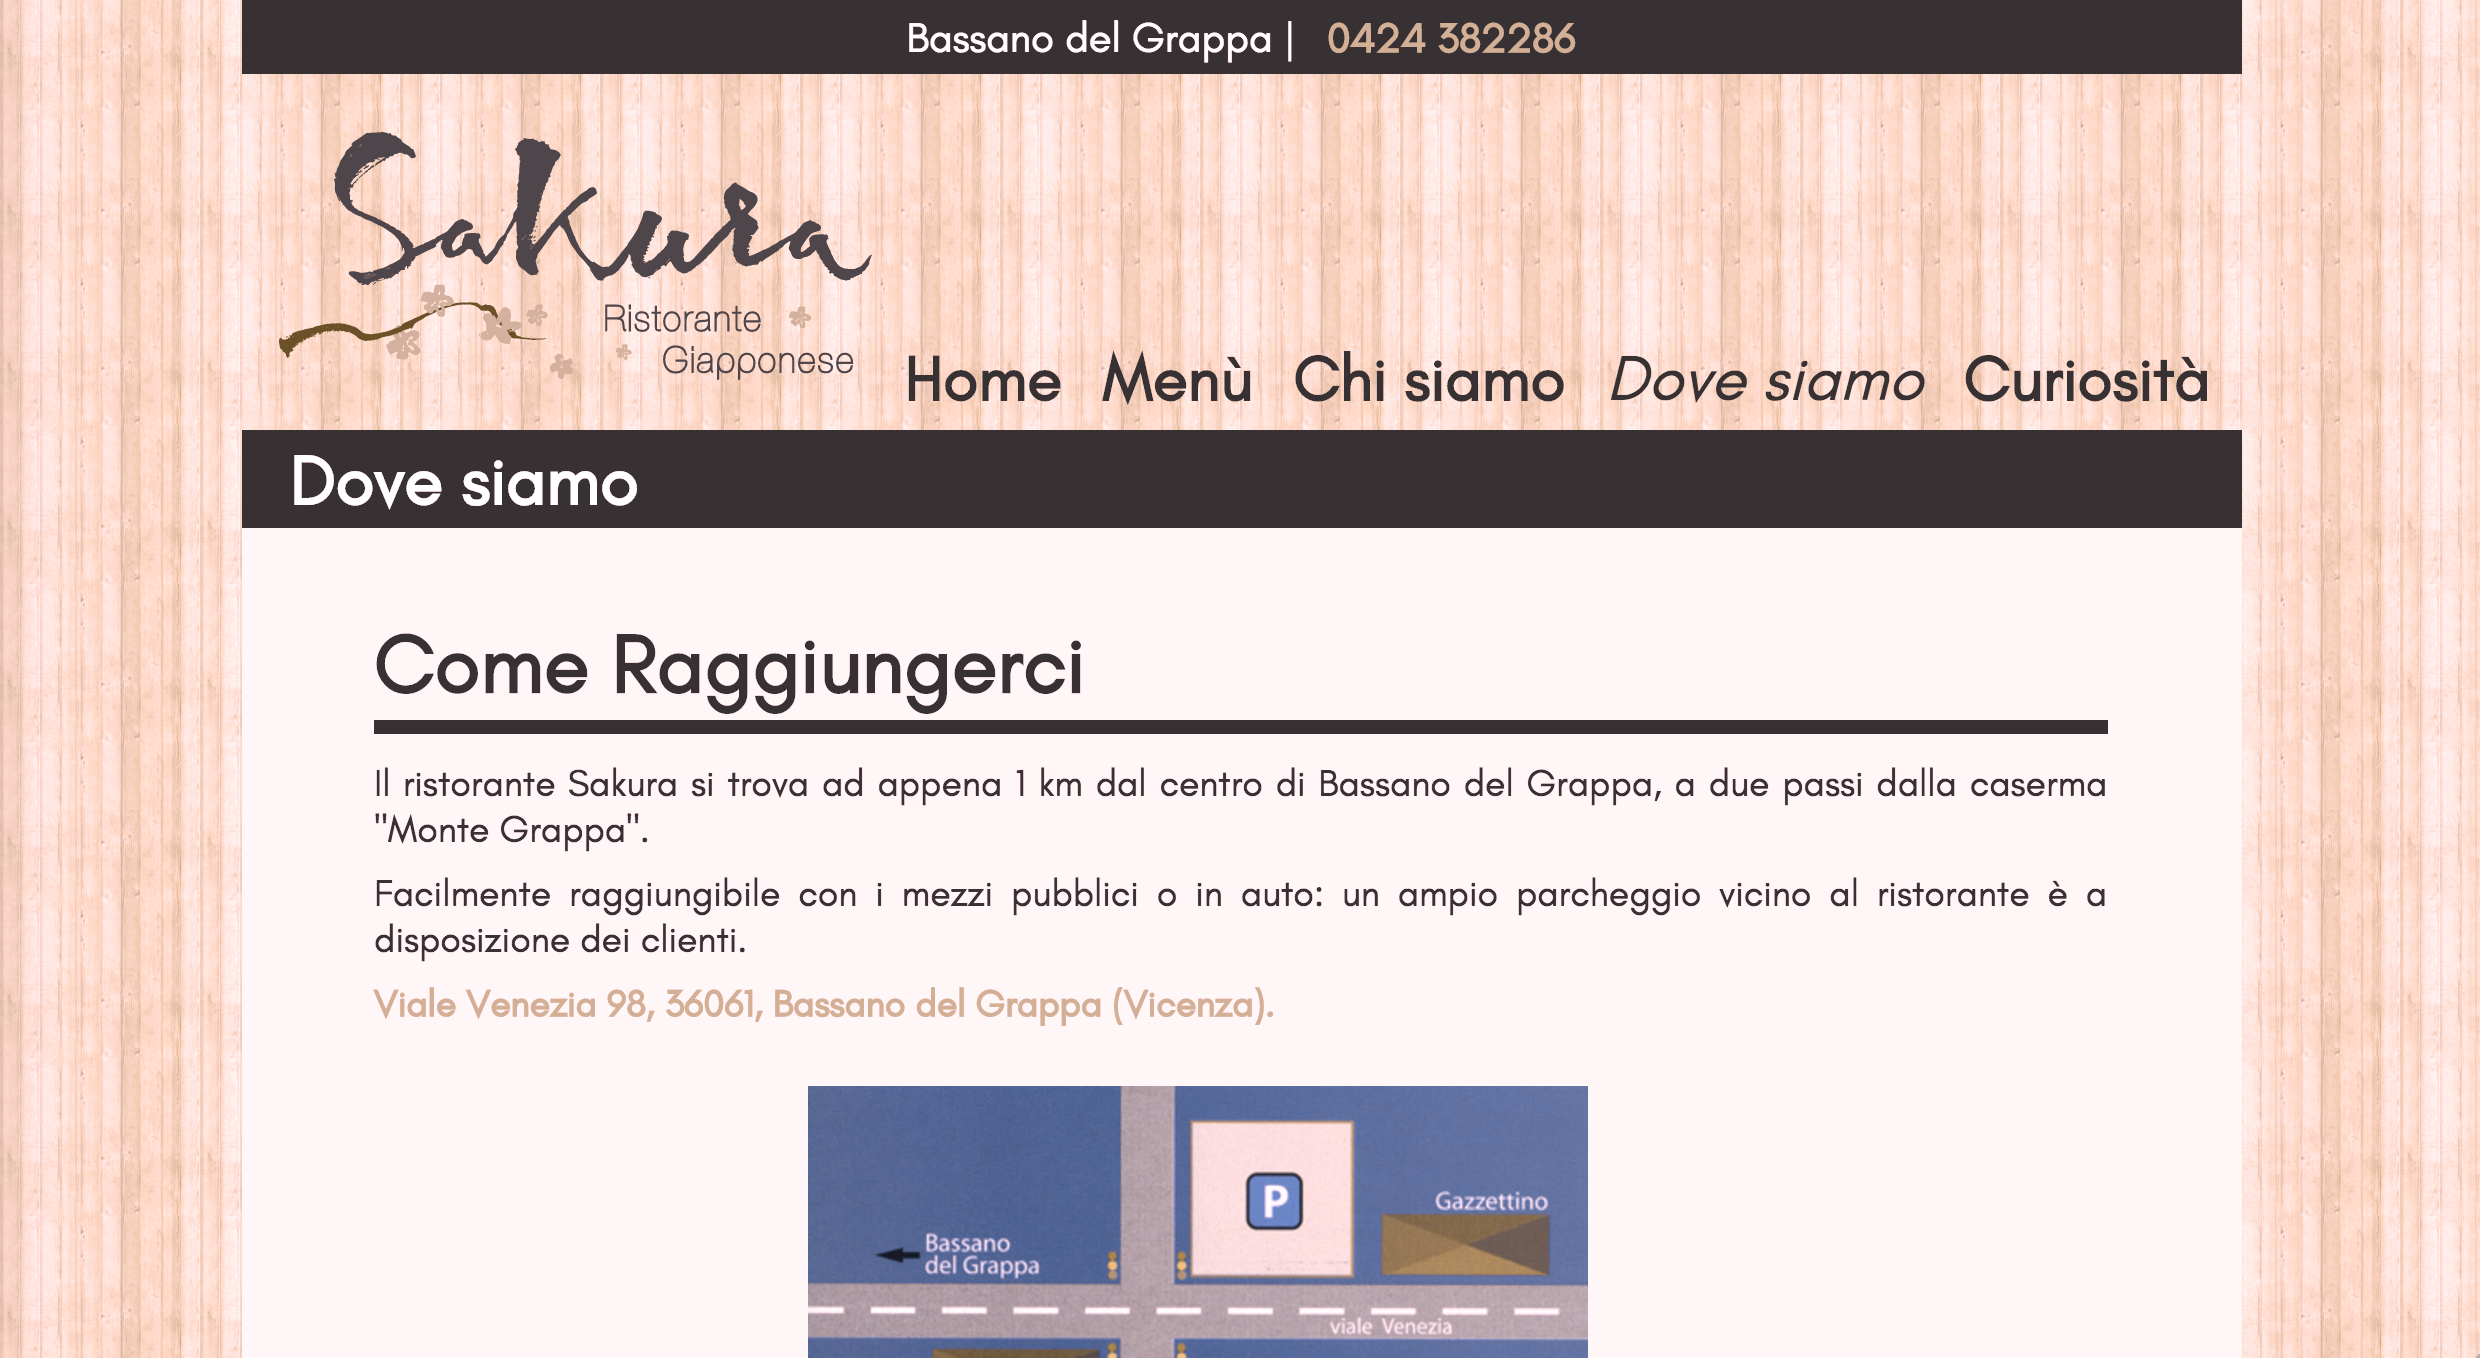
\includegraphics[width=\textwidth]{images/colorblindness/deuteranopia}
		\caption{Esempio di pagina vista da chi soffre di deuteranopia}
		\label{fig:Esempio di pagina vista da chi soffre di deuteranopia}
	\end{figure}
	\begin{figure}[H]
	\centering
		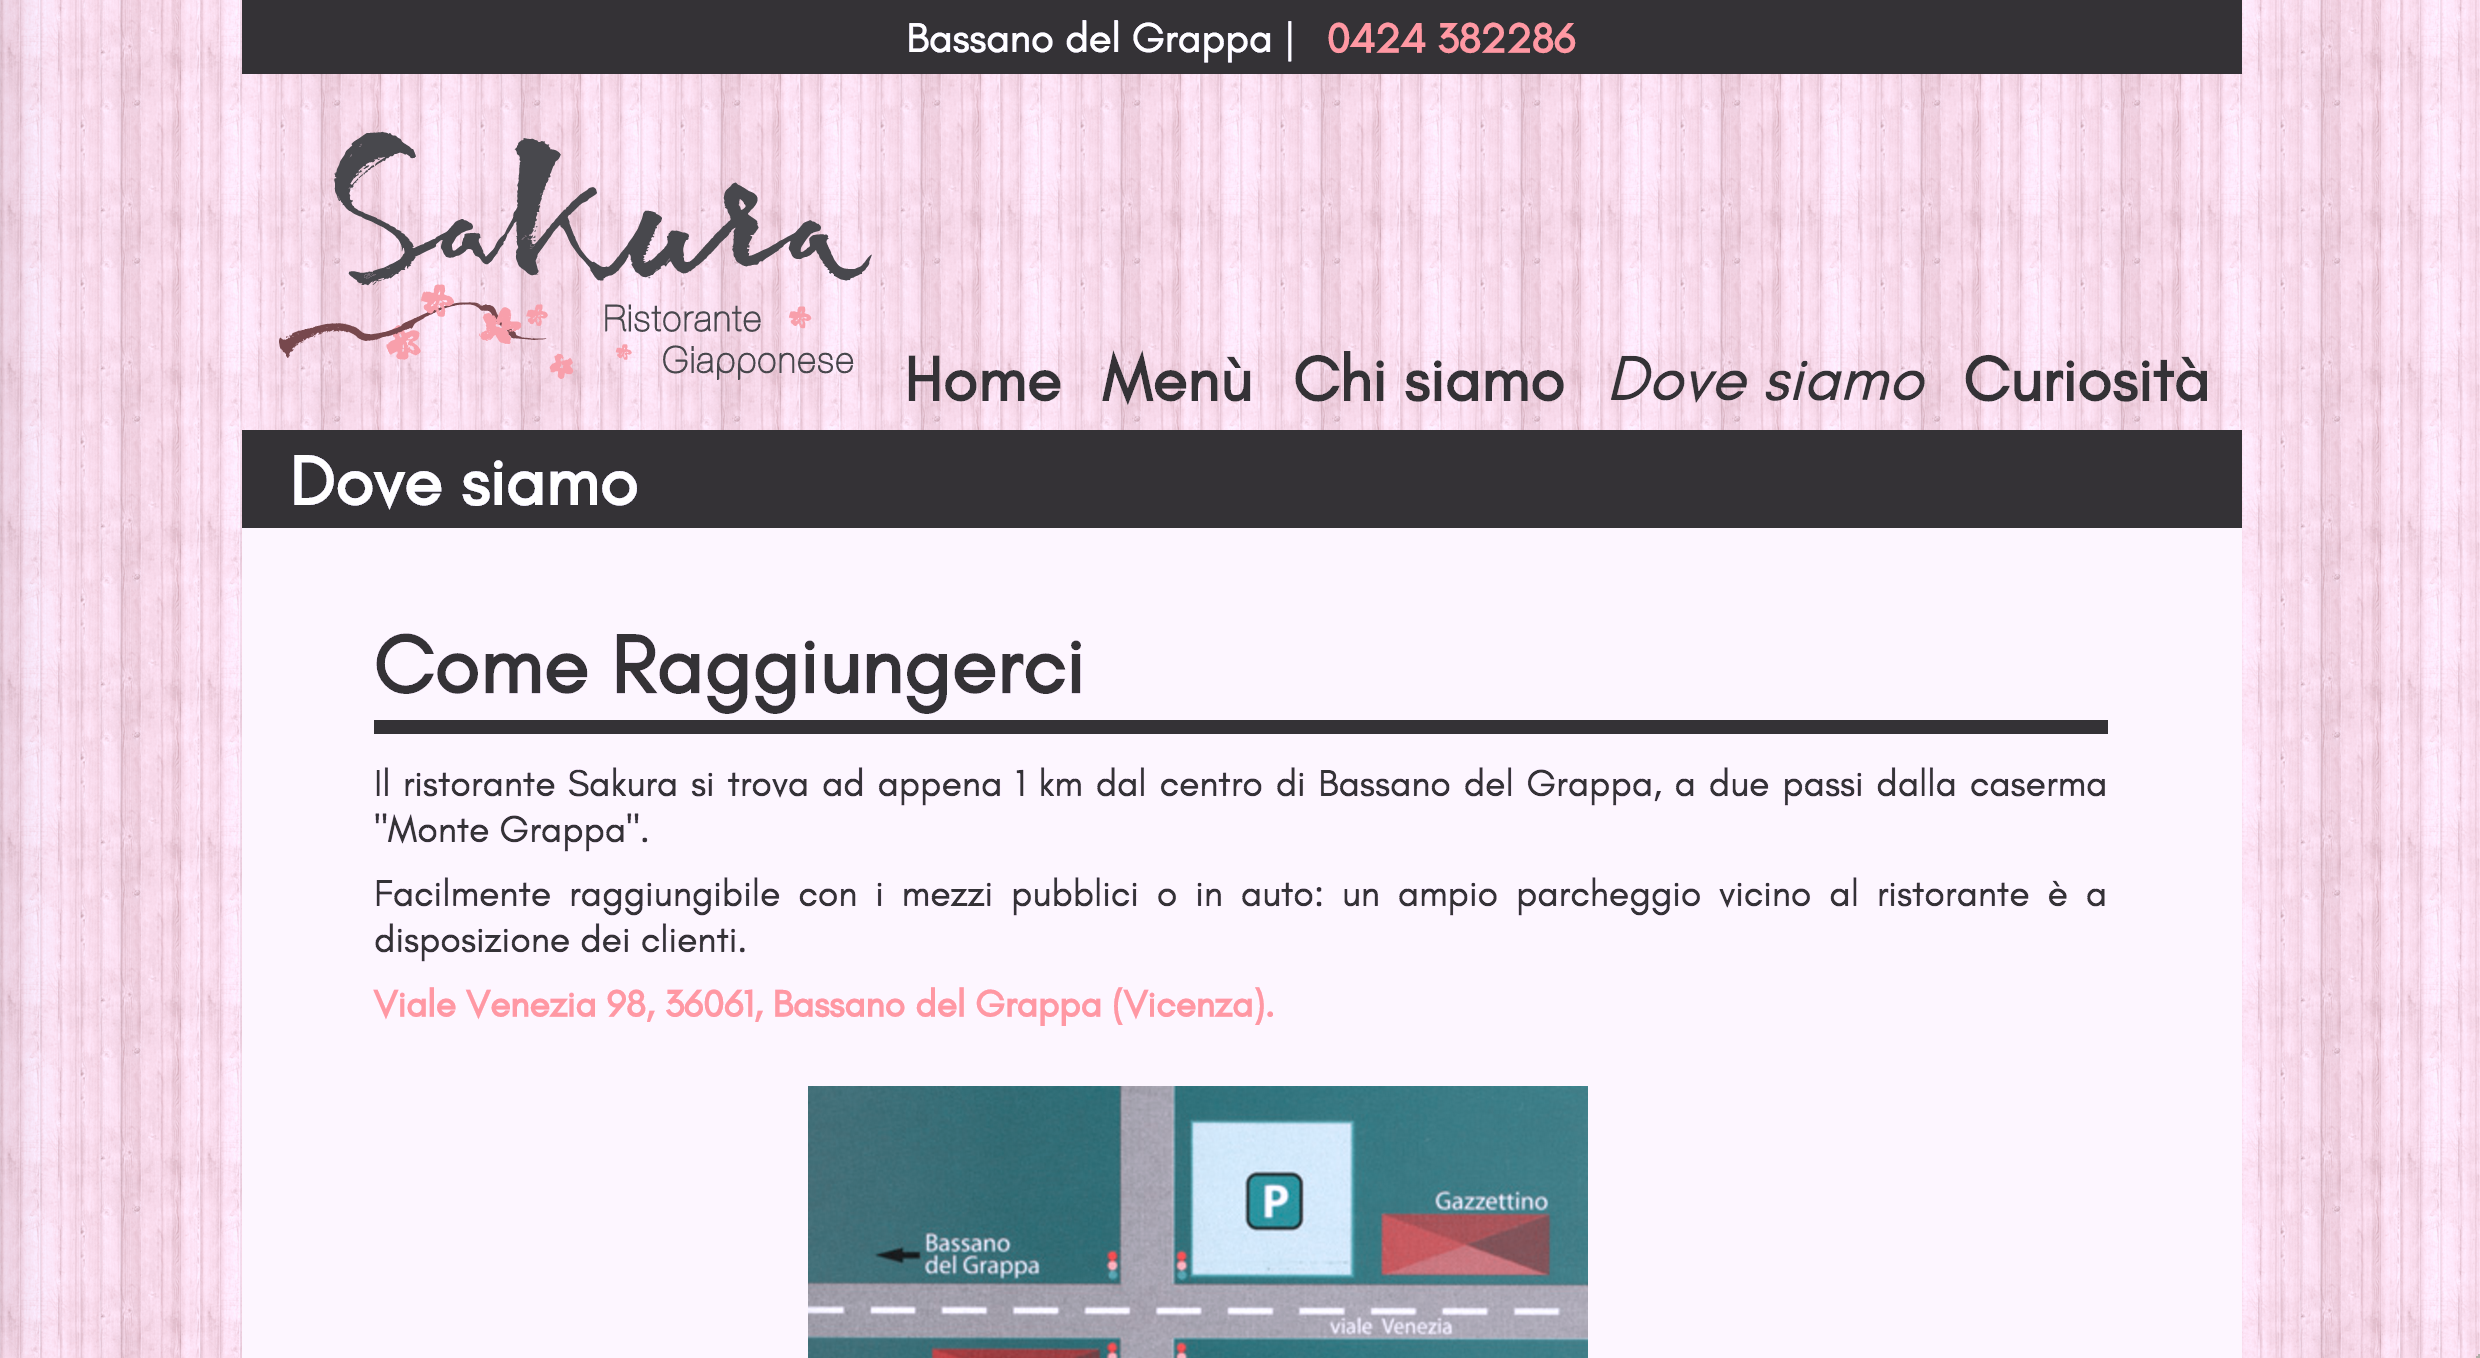
\includegraphics[width=\textwidth]{images/colorblindness/tritanopia}
		\caption{Esempio di pagina vista da chi soffre di tritanopia}
		\label{fig:Esempio di pagina vista da chi soffre di tritanopia}
	\end{figure}
	\begin{figure}[H]
	\centering
		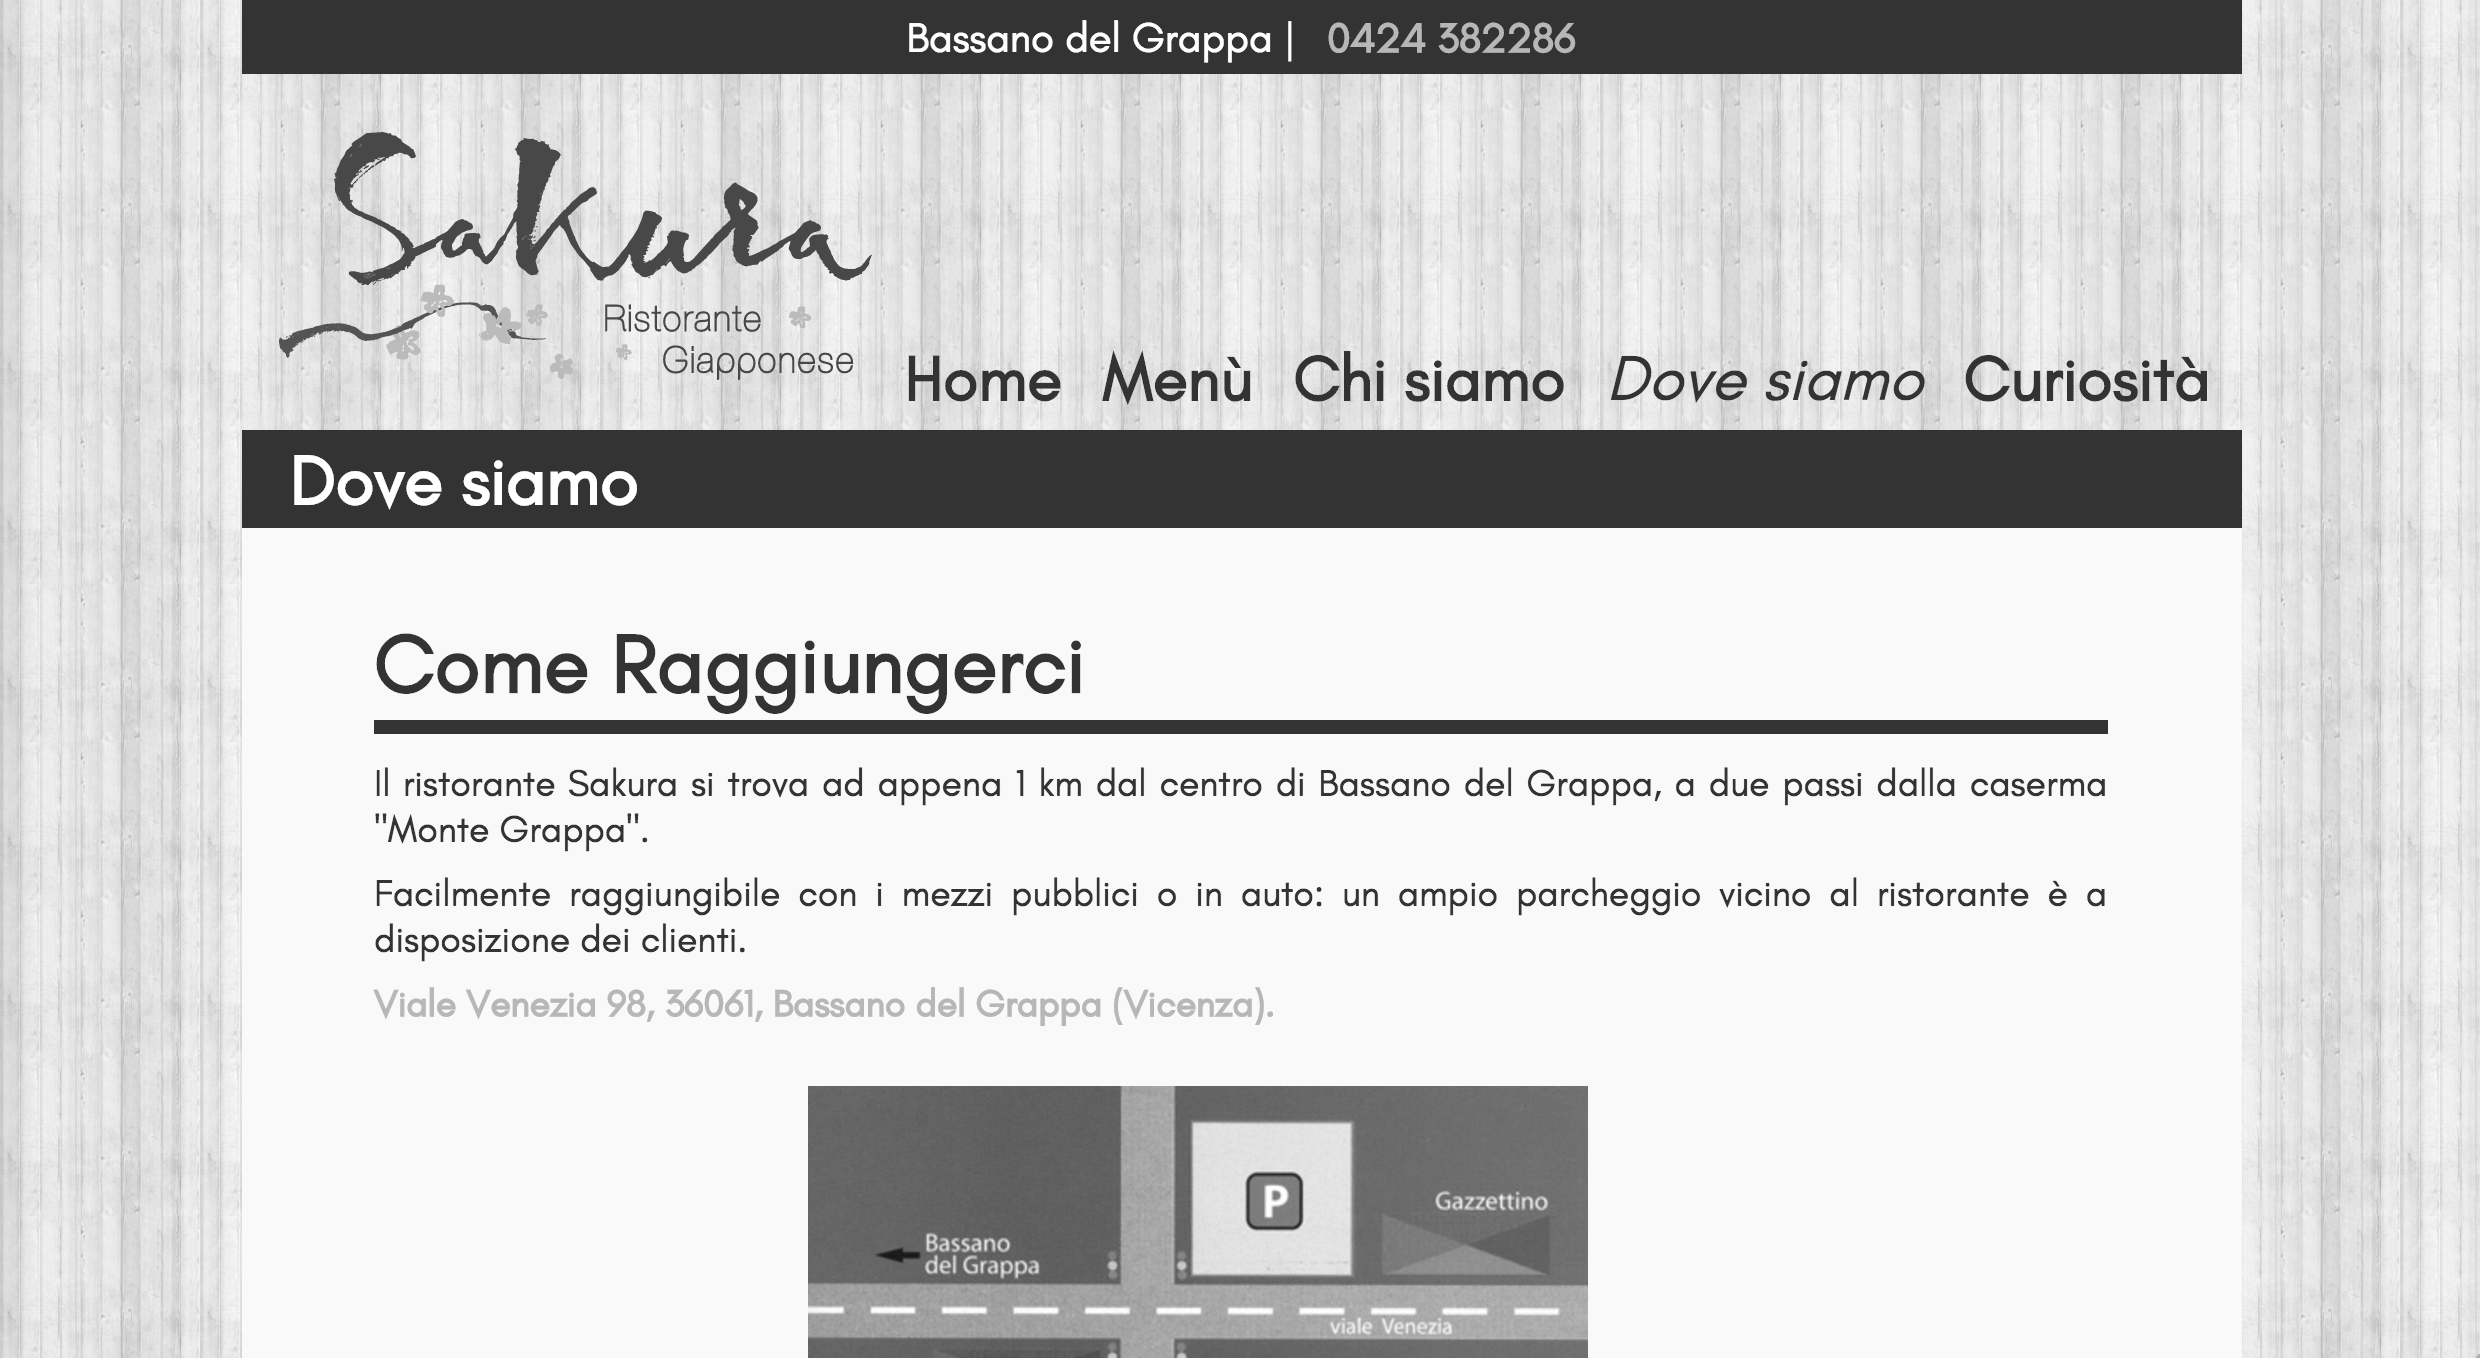
\includegraphics[width=\textwidth]{images/colorblindness/monochromacy}
		\caption{Esempio di pagina vista da chi soffre di monochromacy}
		\label{fig:Esempio di pagina vista da chi soffre di monochromacy}
	\end{figure}
\end{document}